% Options for packages loaded elsewhere
\PassOptionsToPackage{unicode}{hyperref}
\PassOptionsToPackage{hyphens}{url}
\documentclass[
  9pt,
  ignorenonframetext,
]{beamer}
\newif\ifbibliography
\usepackage{pgfpages}
\setbeamertemplate{caption}[numbered]
\setbeamertemplate{caption label separator}{: }
\setbeamercolor{caption name}{fg=normal text.fg}
\beamertemplatenavigationsymbolsempty
% remove section numbering
\setbeamertemplate{part page}{
  \centering
  \begin{beamercolorbox}[sep=16pt,center]{part title}
    \usebeamerfont{part title}\insertpart\par
  \end{beamercolorbox}
}
\setbeamertemplate{section page}{
  \centering
  \begin{beamercolorbox}[sep=12pt,center]{section title}
    \usebeamerfont{section title}\insertsection\par
  \end{beamercolorbox}
}
\setbeamertemplate{subsection page}{
  \centering
  \begin{beamercolorbox}[sep=8pt,center]{subsection title}
    \usebeamerfont{subsection title}\insertsubsection\par
  \end{beamercolorbox}
}
% Prevent slide breaks in the middle of a paragraph
\widowpenalties 1 10000
\raggedbottom
\AtBeginPart{
  \frame{\partpage}
}
\AtBeginSection{
  \ifbibliography
  \else
    \frame{\sectionpage}
  \fi
}
\AtBeginSubsection{
  \frame{\subsectionpage}
}
\usepackage{iftex}
\ifPDFTeX
  \usepackage[T1]{fontenc}
  \usepackage[utf8]{inputenc}
  \usepackage{textcomp} % provide euro and other symbols
\else % if luatex or xetex
  \usepackage{unicode-math} % this also loads fontspec
  \defaultfontfeatures{Scale=MatchLowercase}
  \defaultfontfeatures[\rmfamily]{Ligatures=TeX,Scale=1}
\fi
\usefonttheme[]{serif}
\usepackage[]{mathpazo}
\ifPDFTeX\else
  % xetex/luatex font selection
\fi
% Use upquote if available, for straight quotes in verbatim environments
\IfFileExists{upquote.sty}{\usepackage{upquote}}{}
\IfFileExists{microtype.sty}{% use microtype if available
  \usepackage[]{microtype}
  \UseMicrotypeSet[protrusion]{basicmath} % disable protrusion for tt fonts
}{}
\makeatletter
\@ifundefined{KOMAClassName}{% if non-KOMA class
  \IfFileExists{parskip.sty}{%
    \usepackage{parskip}
  }{% else
    \setlength{\parindent}{0pt}
    \setlength{\parskip}{6pt plus 2pt minus 1pt}}
}{% if KOMA class
  \KOMAoptions{parskip=half}}
\makeatother
\usepackage{graphicx}
\makeatletter
\newsavebox\pandoc@box
\newcommand*\pandocbounded[1]{% scales image to fit in text height/width
  \sbox\pandoc@box{#1}%
  \Gscale@div\@tempa{\textheight}{\dimexpr\ht\pandoc@box+\dp\pandoc@box\relax}%
  \Gscale@div\@tempb{\linewidth}{\wd\pandoc@box}%
  \ifdim\@tempb\p@<\@tempa\p@\let\@tempa\@tempb\fi% select the smaller of both
  \ifdim\@tempa\p@<\p@\scalebox{\@tempa}{\usebox\pandoc@box}%
  \else\usebox{\pandoc@box}%
  \fi%
}
% Set default figure placement to htbp
\def\fps@figure{htbp}
\makeatother
\setlength{\emergencystretch}{3em} % prevent overfull lines
\providecommand{\tightlist}{%
  \setlength{\itemsep}{0pt}\setlength{\parskip}{0pt}}
% Document Class options:
% - You can use article(beamer) or presentation(beamer)
% - In presentation, you can use following options:
%    'trans' for transparent, 'handout' for printing-friendly version
%    'notes' also output notes, 'notesonly' only output notes

% If you have several lectures defined in the same document, uncomment this:
%\includeonlylecture{cours02}

\usepackage{fontspec}
%\fontfamily{ppl}\selectfont
\setmainfont{Arial}
%\setmainfont{DejaVu LGC Sans}
%\setmainfont[SmallCapsFont=Fontin SmallCaps]{Fontin-Regular}
%\setmainfont{Gentium Basic}
%\setsansfont{DejaVu LGC Sans}
%\setmonofont{DejaVu LGC Sans Mono}
%\setmainfont{Calibri}
%\setmainfont{Cambria}
%\setsansfont{Candara}
%\setmonofont{Consolas}

% UMONS-EcoNum template configuration
\mode<all>
{
  \definecolor{umons-red}{RGB}{168, 0, 57}
  \definecolor{umons-turquoise}{RGB}{0, 171, 204}
  \definecolor{umons-gray}{RGB}{150, 150, 150}
  \definecolor{umons-gray2}{RGB}{110, 110, 110}
  \usepackage[labelfont=bf, tableposition=top]{caption}
}
\mode<article>
{
  \usepackage{beamerbasearticle}
  \usepackage{fullpage}
  \pdfimageresolution 96
}
\mode<beamer>
{
  % Customizable items (make sure corresponding pictures are in /template subdir):
  % The background image
  \usebackgroundtemplate{\includegraphics[width=1.07\paperwidth,
height=1.07\paperheight]{../../template/background-hex.jpg}}
  % The logo picture
  \logo{\includegraphics[width=2cm]{../../template/UMONS-logo.pdf}}
}
\mode<handout>
{
  \definecolor{umons-red}{RGB}{84, 84, 84}
  \definecolor{umons-turquoise}{RGB}{168, 168, 168}
  \usepackage{pgfpages}
  \pgfpagesuselayout{2 on 1}[a4paper, border shrink=5mm]
}
\mode<presentation>
{
  % General theme to use
  \usetheme{CambridgeUS}
  %\usetheme{AnnArbor}
  %\usetheme{default}
  %\usetheme{Pittsburgh}
  %\usetheme{Dresden}
  %\usetheme{Hannover}
  % Color theme (but must colors redefined hereunder)
  \usecolortheme{beaver}
  % Theme used for bullets
  \useinnertheme{rectangles}
  %or \useinnertheme{circles}
  % This is to get semi-transparent covered items
  \setbeamercovered{transparent}
  % Rounded rectangular blocks without shadow
  \setbeamertemplate{blocks}[rounded][shadow=false]
 %\usepackage{beamerthemeshadow}

  \setbeamersize{text margin left=1em,text margin right=1em}
  \setbeamerfont{title}{size=\huge}
  \setbeamerfont{subtitle}{size=\large}
  \setbeamerfont{institute}{size=\small}
  \setbeamerfont{date}{size=\small}
  \setbeamerfont{framesubtitle}{size=\small}
  % This stands out a little bit more than umons-red!
  \setbeamercolor{alerted text}{fg=red!80!black}
  %\setbeamercolor{alerted text}{fg=umons-red}
  \setbeamercolor*{palette primary}{fg=black, bg=umons-turquoise}
  \setbeamercolor*{palette secondary}{fg=black, bg=umons-turquoise}
  \setbeamercolor*{palette tertiary}{fg=umons-gray!30, bg=umons-red!80!black}
  \setbeamercolor*{palette quaternary}{fg=black, bg=umons-turquoise}
  \setbeamercolor*{upper separation line head left}{parent=palette tertiary}
  \setbeamercolor*{upper separation line head right}{parent=palette primary}
  \setbeamercolor{title}{fg=umons-red}
  \setbeamercolor*{titlelike}{fg=umons-red}
  \setbeamercolor{institute}{fg=umons-gray2}
  \setbeamercolor{date}{fg=umons-gray2}
  \setbeamercolor{frametitle}{fg=umons-red, bg=white}
  \setbeamercolor{frametitle right}{bg=white}
  \setbeamercolor{structure}{fg=umons-turquoise}
  \setbeamercolor*{separation line}{}
  \setbeamercolor*{fine separation line}{}
  \setbeamercolor*{sidebar}{fg=umons-red,bg=white}
  \setbeamercolor*{palette sidebar primary}{fg=umons-turquoise!10!black}
  \setbeamercolor*{palette sidebar secondary}{fg=umons-red}
  \setbeamercolor*{palette sidebar tertiary}{fg=umons-red!50!black}
  \setbeamercolor*{palette sidebar quaternary}{fg=umons-red}
  \setbeamercolor*{example text}{fg=umons-gray2}

  % Change the footer
  \makeatother
  \setbeamertemplate{footline}
  {
    \leavevmode%
    \hbox{%
    \begin{beamercolorbox}[wd=.35\paperwidth,ht=2.25ex,dp=1ex,center]{author in head/foot}%
      \usebeamerfont{author in head/foot}\insertshortauthor
    \end{beamercolorbox}%
    \begin{beamercolorbox}[wd=.57\paperwidth,ht=2.25ex,dp=1ex,center]{title in head/foot}%
      \usebeamerfont{title in head/foot}\insertshorttitle\hspace*{3em}
    \end{beamercolorbox}%
    \begin{beamercolorbox}[wd=.08\paperwidth,ht=2.25ex,dp=1ex,center]{title in head/foot}%
      \insertframenumber{} / \inserttotalframenumber\hspace*{1ex}
    \end{beamercolorbox}}%
    \vskip0pt%
  }
  \makeatletter
  \setbeamertemplate{navigation symbols}{}

  % Custom Sweave styles
  %\definecolor{SinputColor}{RGB}{25, 25, 125}
  %\definecolor{SoutputColor}{RGB}{110, 110, 110}
  %\DefineVerbatimEnvironment{Sinput}{Verbatim}{fontsize=\small,formatcom=\color{SinputColor}}
  %\DefineVerbatimEnvironment{Soutput}{Verbatim}{fontsize=\small,formatcom=\color{SoutputColor}}
  %\DefineVerbatimEnvironment{Scode}{Verbatim}{fontsize=\small,\color{SinputColor}}
}

% To get coherent font between text and equations
\usefonttheme{professionalfonts}
%\usepackage{mathpazo}
% Useful package in this context
\usepackage{listings}
% Command used to place a picture somewhere in the slide (relative to current pos)
\newcommand{\putat}[3]{\begin{picture}(0,0)(0,0)\put(#1,#2){#3}\end{picture}}

% Idem, but in absolute pos (slide = 128x96mm)
\usepackage{textpos}
\newcommand{\putabs}[3]{\begin{textblock*}{10mm}[0,0](#1,#2){#3}\end{textblock*}}

% Commands useful to place columns in the slides
\newcommand{\columnsbegin}{\begin{columns}}
\newcommand{\columnsend}{\end{columns}}
\newcommand{\columnhalf}{\column{.5\textwidth}}
\newcommand{\columnlarge}{\column{.66\textwidth}}
\newcommand{\columnsmall}{\column{.33\textwidth}}
\newcommand{\columnverylarge}{\column{.75\textwidth}}
\newcommand{\columnverysmall}{\column{.25\textwidth}}

% Copyright notices and sources:
% The background picture: http://www.uberpiglet.com/vectors/20-amazing-vector-backgrounds/
% UMONS-EcoNum template is partly inspired from a work done by:
% C. Troestler <Christophe.Troestler@umons.ac.be> licensed under GNU GPL v3 or later.

% SLIDE NOTES:
% For slide notes, use the \note{} beamer style in your document.
% To make sure to generate note pages even where there are no notes
% (in order to have side-by-side slides at left and notes at right),
% we add this:
\makeatletter
\def\beamer@framenotesbegin{%
  \gdef\beamer@noteitems{}%
  \gdef\beamer@notes{{}}%
}
\makeatother
% Uncomment this line to print notes:
%\setbeameroption{show notes}
% To interleave slides and notes in the PDF:
%\setbeamertemplate{note page}[plain]
% To get only notes:
%\setbeameroption{show only notes}

% Uncomment the following 3 lines in presentation mode for dual screen
% use (and specify 'left', 'top', 'right' or 'bottom' for second screen...)
%\usepackage{pgfpages}
%\setbeameroption{second mode text on second screen=right}
%\setbeameroption{show notes on second screen}

% More packages and options
\usepackage{graphicx}
\usepackage{rotating}
%\setbeamertemplate{caption}[numbered]
\usepackage{hyperref}
\usepackage[normalem]{ulem}
%\mode<presentation>
\usepackage{wasysym}
%\usepackage{amsmath}

% Redefine colors for links
\hypersetup{colorlinks=true,urlcolor=umons-red,linkcolor=umons-red,% link color controls section, subsection, and title
citecolor = umons-red, anchorcolor = umons-red}
% We do not want to change link colors in infolines
\addtobeamertemplate{headline}{\hypersetup{allcolors=.}}{}
\addtobeamertemplate{footline}{\hypersetup{allcolors=.}}{}

% Do not print slides with first level header
\AtBeginSection[]{}

% Redefine how subsection slides appear
\AtBeginSubsection{
  \frame{
    \centering
    \LARGE
    \insertsubsection
  }
}
\usepackage{bookmark}
\IfFileExists{xurl.sty}{\usepackage{xurl}}{} % add URL line breaks if available
\urlstyle{same}
% fallback for those not using the hyperref driver hyperxmp:
\makeatletter
\@ifundefined{xmpquote}{\newcommand{\xmpquote}[1]{#1}}{}
\makeatother
\hypersetup{
  pdftitle={Science des données I},
  pdfauthor={Philippe Grosjean \& Guyliann Engels},
  hidelinks,
  pdfcreator={LaTeX via pandoc}}

\title{\texorpdfstring{Science des données I}{Science des données I}}
\subtitle{\texorpdfstring{\includegraphics[width=.08\textwidth,height=.1\textheight]{../../template/biodatascience.png}
\includegraphics[width=.08\textwidth,height=.1\textheight]{../../template/SciViews-logo.pdf}
\vfill First class meeting}{  First class meeting}}
\author{\texorpdfstring{Philippe Grosjean \& Guyliann
Engels}{Philippe Grosjean \& Guyliann Engels}}
\date{}
\institute{Université de Mons, Belgique\break Service d'Écologie
numérique\break \includegraphics[width=.08\textwidth,height=.1\textheight]{../../template/EcoNum-logo.pdf}
\break \url{https://wp.sciviews.org} \break \url{sdd@sciviews.org}}

\begin{document}
\frame{\titlepage}

\subsection{Organisation de la salle}\label{organisation-de-la-salle}

\begin{frame}{Organisation de la salle}
\begin{itemize}
\item
  Se placer par quatre par rangée (groupe de travail, même place toute
  l'année)
\item
  Allumer son ordinateur ou l'ordinateur de la salle (un par étudiant)
\item
  Utiliser un câble ethernet à la place du wifi (plus rapide)
\item
  Se munir d'un post-it jaune pour les questions
\item
  Remplir les questionnaires sur les tables
\end{itemize}
\end{frame}

\subsection{Qui sommes nous ?}\label{qui-sommes-nous}

\begin{frame}{Présentation}
\protect\phantomsection\label{pruxe9sentation}
Philippe Grosjean, Guyliann Engels
(\href{mailto:sdd@sciviews.org}{\nolinkurl{sdd@sciviews.org}})

\columnsbegin
\columnhalf
\center

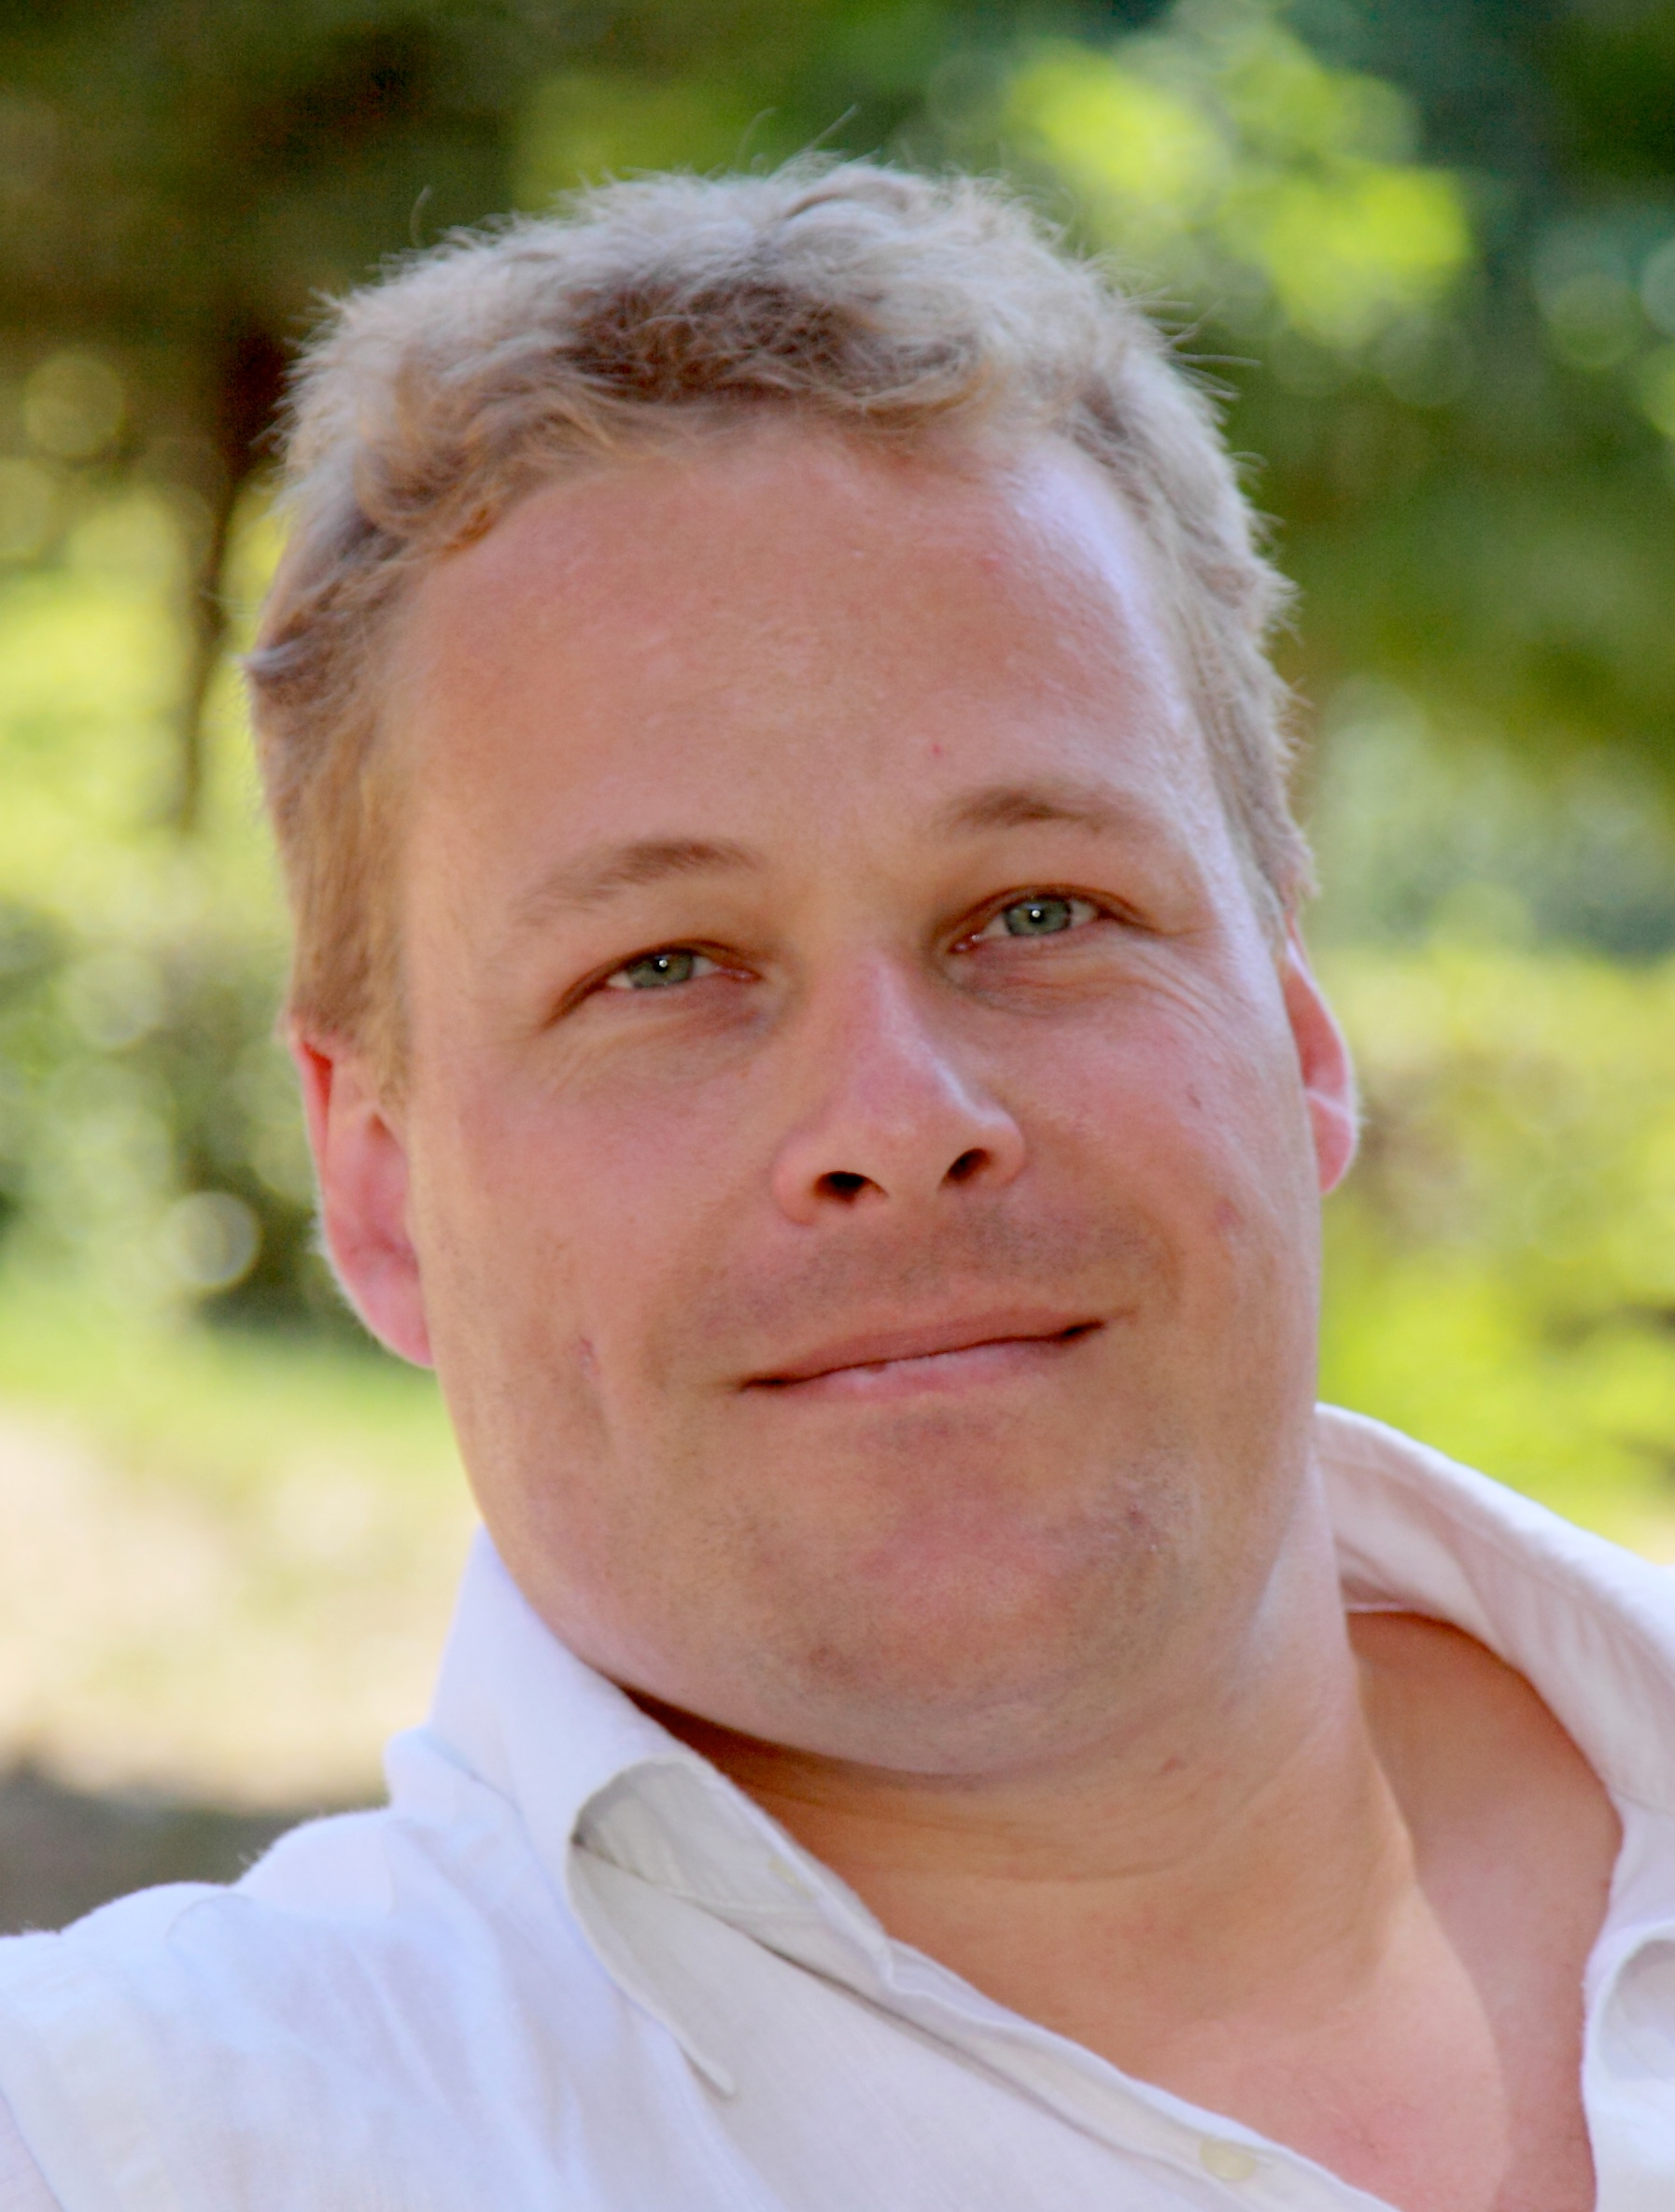
\includegraphics[width=0.85\linewidth]{figures/PhilippeGrosjean}

\columnhalf

\includegraphics[width=0.85\linewidth]{figures/guyliann}

\columnsend
\end{frame}

\subsection{Installation et configuration des
logiciels}\label{installation-et-configuration-des-logiciels}

\begin{frame}{Espace Moodle}
\protect\phantomsection\label{espace-moodle}
\begin{enumerate}
\tightlist
\item
  Accéder au cours sur Moodle \textbf{Science des données I :
  visualisation}
\item
  Cliquer sur l'item \textbf{Lier et aller à wp.sciviews.org}
\item
  Dans le site du cours, cliquer sur ``Home''
\item
  Lire la page
\end{enumerate}
\end{frame}

\begin{frame}{Compte GitHub}
\protect\phantomsection\label{compte-github}
Lire la section \emph{Bien débuter\ldots{}} :
\url{https://wp.sciviews.org}

\vfill

Résumé des étapes

\begin{enumerate}
\tightlist
\item
  Choisir un identifiant GitHub (PrenomNom, éventuellement abbrégé et
  sans accents ou caractères spéciaux) et le faire valider par un
  enseignant
\item
  Créer son compte GitHub
\item
  Cliquer sur ``Login GitHub'' dans le cours pour s'y identifier
\end{enumerate}
\end{frame}

\begin{frame}{Compte Saturn Cloud}
\protect\phantomsection\label{compte-saturn-cloud}
Cliquer sur le bouton bleu \textbf{RStudio} en haut à droite dans le
site du cours pour les instructions d'installation.

\vfill

Résumé des étapes

\begin{enumerate}
\tightlist
\item
  Invitation par mail -\textgreater{} rejoindre l'organisation Econum de
  Saturn Cloud
\item
  Générer la clé ssh sur Saturn Cloud
\item
  Ajouter la clé ssh dans GitHub
\item
  Invitation par mail -\textgreater{} rejoindre Posit Connect
\item
  Générer une API KEY sur Posit Connect
\item
  Créer un nouveau secret dans son compte Saturn Cloud pour l'API KEY
\item
  Créer sa ressource svbox2026sdd
\end{enumerate}
\end{frame}

\subsection{Science des données}\label{science-des-donnuxe9es}

\begin{frame}{Science des données : une approche pragmatique}
\protect\phantomsection\label{science-des-donnuxe9es-une-approche-pragmatique}
\pandocbounded{\includegraphics[keepaspectratio]{A00Pa_intro_files/figures/data-scientist-useful.jpg}}
\end{frame}

\begin{frame}{Science des données : à l'interface entre plusieurs
disciplines}
\protect\phantomsection\label{science-des-donnuxe9es-uxe0-linterface-entre-plusieurs-disciplines}
\columnsbegin
\columnhalf

\begin{itemize}
\item
  La Science des Données, c'est la discipline qui s'intéresse à
  l'analyse de données \emph{sous toutes ses formes}
\item
  Très large et \textbf{interdisciplinaire} :

  \begin{itemize}
  \tightlist
  \item
    \textbf{(Bio)statistiques} et visualisation
  \item
    Utilisation d'\textbf{outils informatiques}
  \item
    Expertise dans le domaine (\textbf{biologie})
  \end{itemize}
\item
  \alert{Il faut maîtriser simultanément les trois domaines pour être un scientifique des données.}
\end{itemize}

\columnhalf

\pandocbounded{\includegraphics[keepaspectratio]{A00Pa_intro_files/figures/data-science-venn.png}}

\columnsend
\end{frame}

\begin{frame}{Pourquoi la science des données ?}
\protect\phantomsection\label{pourquoi-la-science-des-donnuxe9es}
\begin{itemize}
\tightlist
\item
  Besoin issu de la \textbf{quantité de données} disponibles (1
  zettabyte = 1 milliard de terabytes = 1 000 000 000 000 000 000 000
  octets).
  \pandocbounded{\includegraphics[keepaspectratio]{A00Pa_intro_files/figures/data-growth.png}}
\end{itemize}
\end{frame}

\subsection{Comment se déroule un
cours~?}\label{comment-se-duxe9roule-un-cours}

\begin{frame}{Cours \emph{ex cathedra} + Travaux pratiques}
\protect\phantomsection\label{cours-ex-cathedra-travaux-pratiques}
\pandocbounded{\includegraphics[keepaspectratio]{A00Pa_intro_files/figures/organisation1.png}}

\begin{itemize}
\item
  Le réel apprentissage se déroule \textbf{après} les séances de cours
  et d'exercices
\item
  Un examen est nécessaire pour vérifier vos acquis
\end{itemize}

D'après la science lors d'un cours \emph{ex cathedra}, \textbf{vous
n'apprenez rien}

-\textgreater{} Quelle perte de temps :(
\end{frame}

\begin{frame}{Pédagogie active et classe inversée}
\protect\phantomsection\label{puxe9dagogie-active-et-classe-inversuxe9e}
\textbf{Cours classique \emph{ex cathedra} + séances d'exercices}

\pandocbounded{\includegraphics[keepaspectratio]{A00Pa_intro_files/figures/organisation1.png}}

\textbf{Approche en classe inversée}

\pandocbounded{\includegraphics[keepaspectratio]{A00Pa_intro_files/figures/organisation2.png}}

\begin{itemize}
\item
  \emph{Aucune} séance en présentiel sans préparation
\item
  Chaque heure de travail pleinement consacrée à l'apprentissage
\item
  Vous êtes actifs \textbf{tout le temps} et vous gérez \textbf{à votre
  rythme}
\item
  \textbf{Pas besoin d'un examen à la fin}~: travail évalué durant
  l'année
\end{itemize}
\end{frame}

\begin{frame}{C'est quoi la classe inversée~?}
\protect\phantomsection\label{cest-quoi-la-classe-inversuxe9e}
\pandocbounded{\includegraphics[keepaspectratio]{A00Pa_intro_files/figures/classe inversee.png}}
\href{https://www.youtube.com/watch?v=uLKmLDrGyjw}{(lien vers la vidéo)}
\end{frame}

\begin{frame}{Classe inversée et pédagogie active}
\protect\phantomsection\label{classe-inversuxe9e-et-puxe9dagogie-active}
Notre approche~: \textbf{pédagogie active en classe inversée} (vous
apprenez \emph{d'abord} à la maison, nous appliquons \emph{ensuite} en
présentiel).

\vfill

\begin{quote}
I \textbf{hear} and I forget.
\end{quote}

\begin{quote}
I \textbf{see} and I remember.
\end{quote}

\begin{quote}
I \textbf{do} and I understand.
\end{quote}

\begin{quote}
--- Confucius
\end{quote}
\end{frame}

\begin{frame}{C'est quoi la pédagogie active~?}
\protect\phantomsection\label{cest-quoi-la-puxe9dagogie-active}
\pandocbounded{\includegraphics[keepaspectratio]{A00Pa_intro_files/figures/pédagogies actives.png}}
\href{https://www.youtube.com/watch?v=ygjSle9Pkg4}{(lien vers la vidéo)}
\end{frame}

\begin{frame}{Et moi, je fais quoi dans tout cela~?}
\protect\phantomsection\label{et-moi-je-fais-quoi-dans-tout-cela}
\center

\includegraphics[width=2.08333in,height=\textheight,keepaspectratio]{A00Pa_intro_files/figures/lisez.jpg}

\begin{itemize}
\item
  Vous êtes \textbf{acteur de votre apprentissage}, les enseignants sont
  des \textbf{facilitateurs} (plus en retrait par rapport à l'approche
  classique).
\item
  Plus de séparation entre \textbf{cours théorique} et
  \textbf{exercices}~; vos échanges avec le professeur et l'assistant
  sont similaires.
\item
  \textbf{Vous posez les questions}, et vos enseignants vous répondent
  \textbf{individuellement}.
\end{itemize}
\end{frame}

\begin{frame}{Apprentissage en quatre niveaux}
\protect\phantomsection\label{apprentissage-en-quatre-niveaux}
\includegraphics[width=0.8\linewidth,height=\textheight,keepaspectratio]{A00Pa_intro_files/figures/apprendre2.png}
\end{frame}

\begin{frame}{Évaluation continue \& planning}
\protect\phantomsection\label{uxe9valuation-continue-planning}
\begin{itemize}
\item
  Le
  \href{https://wp.sciviews.org/sdd-umons2/?iframe=wp.sciviews.org/sdd-umons-2026/planning-des-s\%25C3\%25A9ances.html}{planning
  des séances} est synthétisé dans le cours en ligne
\item
  Suivi de votre progression dans
  \href{https://moodle.umons.ac.be}{Moodle} ou à la fin de chaque module
  du cours
\item
  Vous aurez des projets (analyse de données biologiques) en séance
\item
  Vous aurez quatre interrogations écrites par AA et un challenge
\item
  Note de l'AA (voir
  \href{https://github.com/BioDataScience-Course/BioDataScience-Common/tree/2026-2027/docs/plan_de_cours/sdd1_plan_cours_2026-2027.pdf}{plan
  de cours})~:

  \begin{itemize}
  \item
    6\% des points pour les exercices (2\% H5P-Shiny et 4\% tutoriels
    learnr)
  \item
    6\% pour les projets individuels
  \item
    28\% pour les projets de groupe
  \item
    5 x 12\% pour les interrogations
  \end{itemize}
\end{itemize}
\end{frame}

\begin{frame}
\begin{center}
\textbf{Avez-vous des questions ?}
\end{center}

\centering

\includegraphics[width=0.3\linewidth,height=\textheight,keepaspectratio]{A00Pa_intro_files/figures/monkey2.jpg}

\vfill

\textbf{Ressources utiles~:}

\begin{itemize}
\tightlist
\item
  Site web du cours~: \url{http://bds.sciviews.org/}
\item
  Cette présentation~:
  \url{https://github.com/BioDataScience-Course/sdd_lessons/tree/2026-2027/A00/presentations}
\end{itemize}
\end{frame}

\end{document}
